\subsection{Generic Chorus}

Generic chorus algorithm is based on simple idea that copies the original sound and then delay
different copies with different delays and then slightly detune them. The very basic chorus is just
parallel delay lines wich are modulated with low-frequency oscillator (LFO) to get some detuning.

Industry standard chorus is is slighly different and even more simple but better sounding. It consist
of one feedback delay line and one feedforward delay line whose are modulated with LFO as in the 
case of basic chorus. Block diagram of the industry standard chorus is shwn in the figure \ref{fig:inds}
\begin{figure}[ht]
\centering
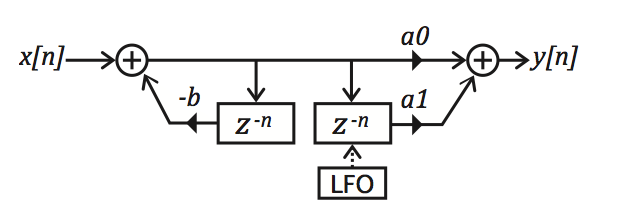
\includegraphics[width = 9cm]{industryStd.png}
\caption{Block diagram of industry standard chorus. \cite{dudas}}
\label{fig:inds}
\end{figure} 

Usually in chorus applications the parameters that can be adusted are not real life related.
Usual parameters are for example modulation depth, modulation speed and feedback gain.
